\documentclass[../main.tex]{subfiles}
\begin{document}

\section{Environment setup}
For evaluation results, all the training processes are conducted on a computer that has an Intel Core i3-9100F CPU and a GTX1660 GPU. However, all the tests are only executed on the Nvidia Jetson Nano Developer Kit which has the technical specifications described in Table~\ref{table:jetson}.

For deployment, each edge node will be a combination of a Jetson Nano, a USB camera, and other peripheral devices. The deployed human feature extraction model was obtained by training with the PRW dataset~\cite{zheng2016person} and the CUHK03 dataset~\cite{li2014deepreid} as described in Section~\ref{subsec:dataset}.

\section{Datasets}
\label{subsec:dataset}
For deployment and evaluation purposes, two public datasets: PRW dataset~\cite{zheng2016person} and CUHK03 dataset~\cite{li2014deepreid} were utilized. Images from these two datasets can be seen in Figure~\ref{fig:prw_cuhk03} with two images on the left from the PRW dataset and two images on the right from the CUHK03 dataset.

\begin{figure}[h!]
\centering
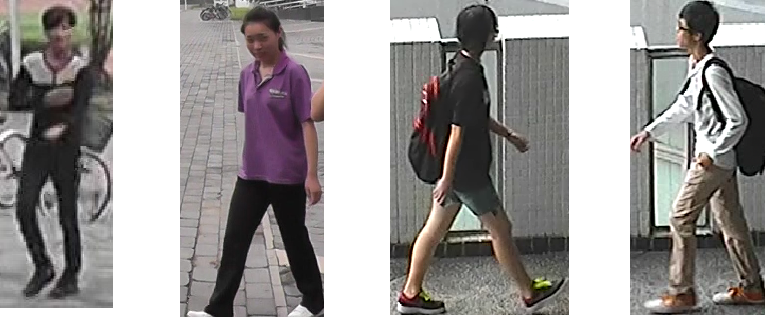
\includegraphics[width=\linewidth]{Figure/prw_cuhk03.pdf}
\caption{Images from PRW and CUHK03 datasets.}
\label{fig:prw_cuhk03}
\end{figure}

\textbf{PRW} dataset~\cite{zheng2016person} was collected using six cameras at Tsinghua University during the summer of 2014. There are a total of 11,816 labeled video frames with 932 identities and 34,304 bounding boxes. This dataset is designed for cross-camera retrieval.

\textbf{CUHK03} dataset~\cite{li2014deepreid} consists of 14,097 pictures of 1,467 individuals, collected using six cameras on campus. Two cameras were used for each individual. There are two types of bounding box annotations in this dataset: manually labeled and automatically labeled using a detector. The dataset contains 20 train/test partitions. Our approach only uses the manually labeled portion of the dataset for training, evaluation, and comparison purposes in any experiments or deployment. 

For evaluation, the feature extraction model was trained and tested only on the CUHK03 dataset because of its popularity. The model was trained for every partition and the final result was averaged from results of 20 partitions. In each partition, 100 identities are separated for testing, 100 identities are split for validation, and the rest are in the training set. The training settings and evaluation results can be seen in Section~\ref{exp:feature}.

For deployment, I combined the data from both of the datasets into one big dataset and use this dataset to train the model. I took out 3,439 images of 100 identities in the PRW dataset for validating purposes and these 100 identities would not appear in the training set. Hyper-parameters and strategy for training are identical to those specified in Section~\ref{subsec:hyper_train}.

\section{Quantitative metrics}
\subsection{IoU}
\label{metric:iou}
IoU stands for Intersection over Union. If there are two bounding boxes, the IoU score of these two bounding boxes is calculated by the intersection of two boxes over the union of them which is shown in Equation~\ref{eq:iou}.

\begin{equation}\label{eq:iou}
    IoU(A, B) = \dfrac {A \cap B} {A \cup B}
\end{equation}
In which:
\begin{outline}
 \1 $A$ and $B$ are bounding boxes.
 \1 $A \cap B$ is the intersection area of two bounding boxes.
 \1 $A \cup B$ is the union area of two bounding boxes.
\end{outline}

\begin{figure}[h!]
\centering
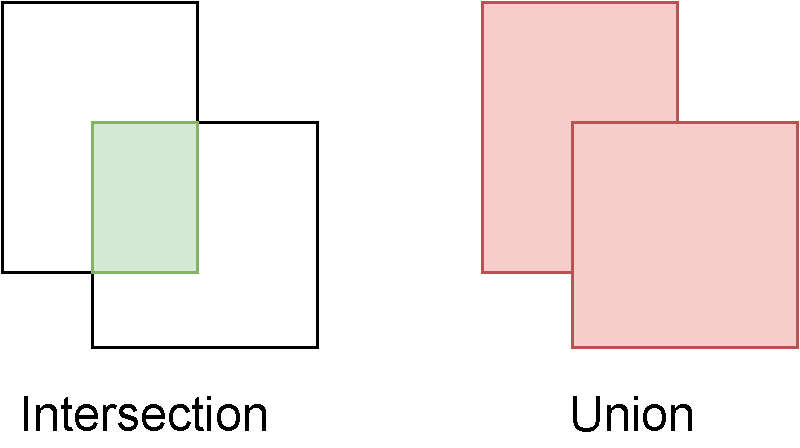
\includegraphics[width=0.6\linewidth]{Figure/IOU.pdf}
\caption{Demonstrations of intersection and union in IoU.}
\label{fig:iou}
\end{figure}

Intersection and union are demonstrated in Figure~\ref{fig:iou}.

\subsection{EER}
\label{metric:eer}
EER stands for Equal Error Rate. EER is a performance metric used to evaluate the accuracy of ReID algorithms in matching pairs of images. EER is the point where the false rejection rate (FRR) and false acceptance rate (FAR) are equal. For example, in a test set, pair-wise distance is calculated for every possible pair of images. Then, the threshold will be adjusted so that the FAR and FRR are equal. At that point, they are also equal to the EER score.

\subsection{Re-ID mAP}
\label{metric:reid_map}
mAP is used in Re-ID algorithms as a performance metric to evaluate the accuracy. It is a measure of how well an algorithm can rank a set of images in order of similarity to a query image.

\begin{figure}[h!]
\centering
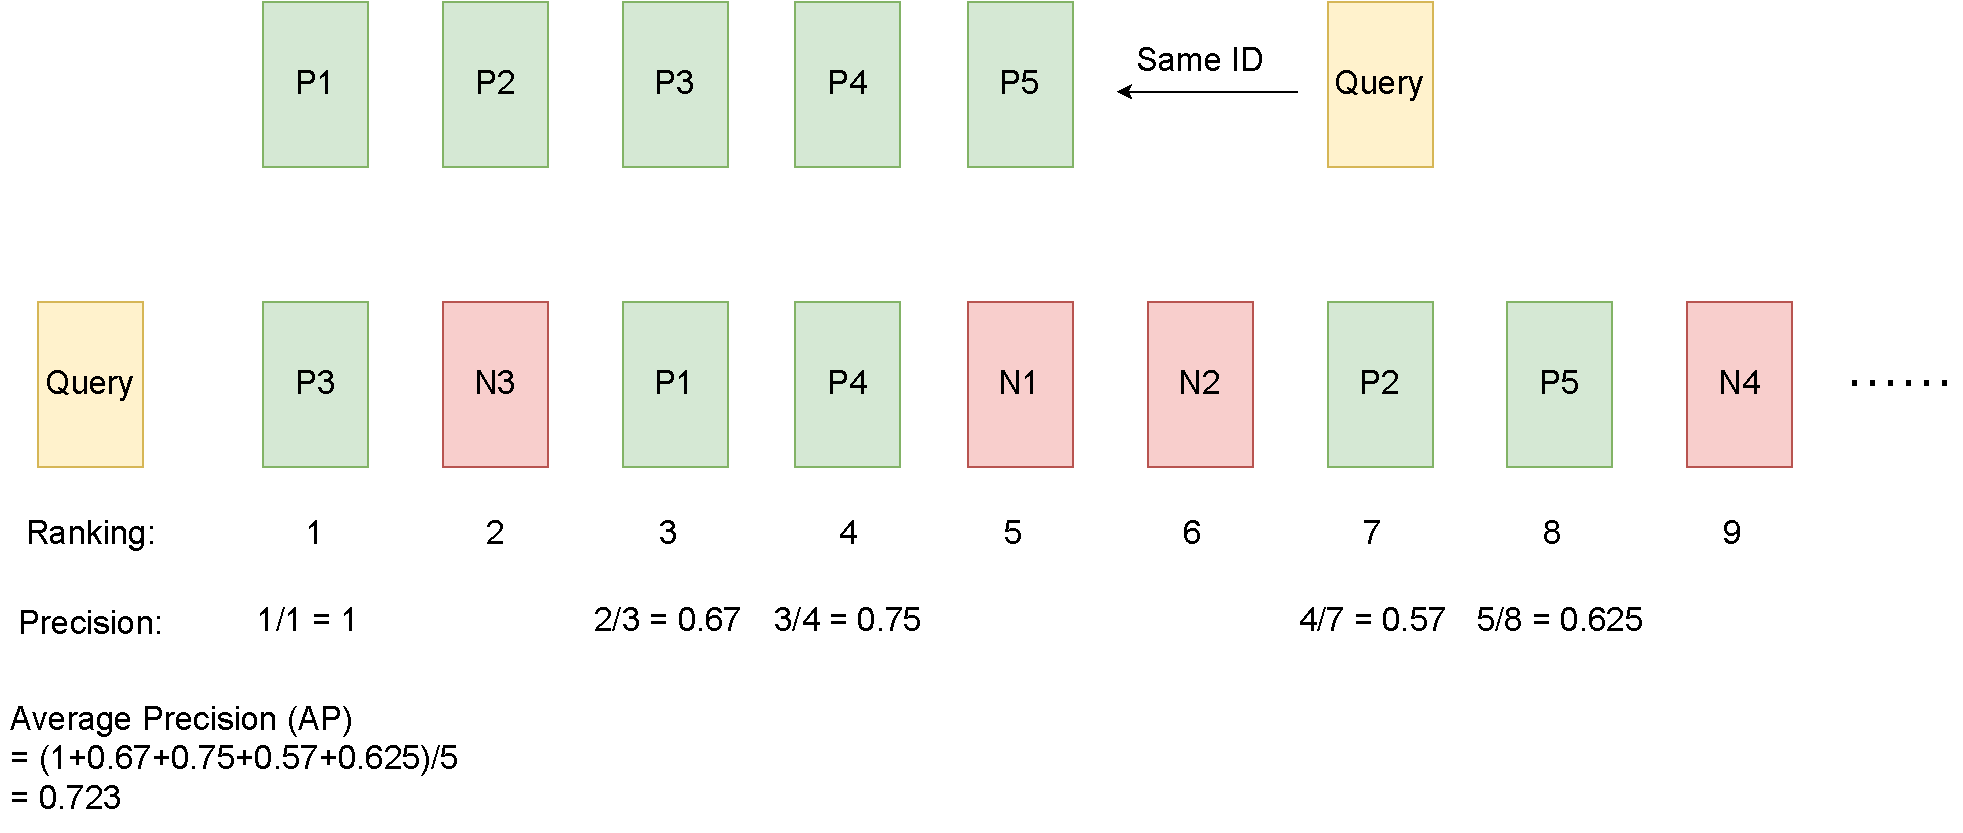
\includegraphics[width=\linewidth]{Figure/reid_map.pdf}
\caption{An example for average precision calculation for a query image. The yellow box is the query sample. Green boxes are samples with the same identity as the query image and red boxes are samples with different identities from the query image.}
\label{fig:reid_map}
\end{figure}

Figure~\ref{fig:reid_map} illustrates the average precision calculation process for a query image. P1 to P5 have the same identity with the query image and N1 to N4 have different identities from the query image. Next, the mean of average precision of all samples in the test set is computed to obtain the final mAP score.
\subsection{Rank-1}
\label{metric:rank-1}
Rank-1 is a performance metric used to evaluate the accuracy of Re-ID algorithms. Rank-1 accuracy measures the percentage of cases where the top-ranked match returned by the algorithm is correct.

Rank-1 accuracy is calculated by comparing the identity of the ground truth query image with the identity of the top-ranked match. Distances between the ground truth query image and all images in the gallery are calculated. Then, the results are sorted by descending the similarity. If the most similar sample in the gallery has the same identity as the query image, this is considered a correct prediction.
The Rank-1 accuracy is the percentage of cases where the algorithm makes a correct prediction for the top-ranked match.

\section{Experimental results of detection model}
Table~\ref{table:detect} shows the evaluation results of detection models on Jetson Nano. Three versions of the model were evaluated. The model is either in the native Pytorch format or in the TensorRT format. TensorRT-converted models were quantized to 16-bit floating points.

\begin{table}[h!]
\centering
\begin{tabular}{||l | c | c | c | c ||} 
\hline 
Model & Input size & \begin{tabular}[c]{@{}l@{}}Converted\\ to TensorRT\end{tabular} & \begin{tabular}[c]{@{}l@{}}Inference time\\ (milliseconds)\end{tabular} \\
\hline
YOLOv5n & $640\times640$ & No & $47.4$ \\
YOLOv5n & $640\times640$ & Yes & $44.1$ \\
YOLOv5n (used in deployment) & $384\times384$ & Yes & $17.9$ \\
\hline
\end{tabular}
\caption{Results of detection models on Jetson Nano.}
\label{table:detect}
\end{table}

As seen in Table~\ref{table:detect}, converting the model to TensorRT format has improved its inference time from $47.4$ milliseconds to $44.1$ milliseconds. Furthermore, if the input size is set to $384\times384$, the inference time of the converted model significantly reduces to $17.9$ milliseconds.

\section{Experimental results of feature extraction model}
\label{exp:feature}

\subsection{Hyper-parameters and training settings}
\label{subsec:hyper_train}
Table~\ref{table:hyperparam} provides a summary of the hyperparameters used in this model. The input was pre-processed to have the size $192\times64$ as described in Section 3.2.2.a. A batch size of $64$ was selected. During the training step, one person from the dataset was chosen, and all samples of this person were added to the mini-batch. The remaining samples in the batch were randomly selected from other people. An epoch ended when all the people in the training set were iterated through. Hard triplet loss with the margin constant of $0.2$ was used. Adam~\cite{kingma2014adam} was utilized as the optimizer with the initial learning rate of $1\times10^{-4}$ The model was trained for $500$ epochs, and the final model was chosen based on the lowest EER score on the validation set.

\begin{table}[h!]
\centering
\begin{tabular}{||c | c | c | c | c ||} 
\hline 
Input size & Batch size & Margin & Initial learning rate & Number of epochs \\
\hline
$192\times64$ & 64 & $0.2$ & $1\times10^{-4}$ & $500$ \\
\hline
\end{tabular}
\caption{Hyperparameters for human feature extraction model.}
\label{table:hyperparam}
\end{table}

\subsection{Evaluation}
Table~\ref{table:reid} shows the experimental results on the CUHK03 dataset. Two versions of the proposed feature extraction model were evaluated. The first model is a native Tensorflow model and the second one is the model which has been converted to TensorRT engine.

\begin{table}[h!]
\centering
\begin{tabular}{||l | c | c | c | c ||} 
\hline 
Model & \begin{tabular}[c]{@{}l@{}}Re-ID mAP\\ (\%)\end{tabular}  & \begin{tabular}[c]{@{}l@{}}Rank-1\\ (\%)\end{tabular} & \begin{tabular}[c]{@{}l@{}}Parameters\\ (millions)\end{tabular} & \begin{tabular}[c]{@{}l@{}}Inference time\\ (milliseconds)\end{tabular} \\
\hline
PCB~\cite{sun2018beyond} & $54.2$ & $61.3$ & $26.8$ & - \\
LightMBN~\cite{herzog2021lightweight} & $85.1$ & $87.2$ & $9.3$ & - \\
Pyramid~\cite{zheng2019pyramidal} & $76.9$ & $78.9$ & $29.1$ & - \\
DSA-reID~\cite{zhang2019densely} & $75.2$ & $78.9$ & $38.5$ & - \\
MPN~\cite{ding2020multi} & $81.1$ & $85.0$ & $31.5$ & - \\
MGN~\cite{wang2018learning} & $67.4$ & $68.0$ & $68.8$ & - \\
\begin{tabular}[c]{@{}l@{}}Customized MobileNetV2 \\(Before conversion)\end{tabular} & $75.7$ & $79.1$ & $0.6$ & $23.4$ \\
\begin{tabular}[c]{@{}l@{}}Customized MobileNetV2 \\(After conversion)\end{tabular} & $75.7$ & $79.1$ & $0.6$ & $4.1$\\
\hline
\end{tabular}
\caption{Results of feature extraction models on the CUHK03 dataset before and after conversion.}
\label{table:reid}
\end{table}

As seen in Table~\ref{table:reid}, while the accuracy of the proposed model is not on par with state-of-the-art models, it is significantly lighter than all other models. In fact, the second-lightest model has about 15 times as many parameters as the proposed model. Despite this, the proposed model still achieves a decent level of accuracy. In addition, without quantization, the precision of both versions of the proposed model is equal. However, the converted model is nearly five times faster than the original model. Moreover, the inference time of the proposed feature extraction model with the original MobileNetV2 backbone is $6.4$ milliseconds. This model is $56\%$ slower than the customized model. When there is only one person in the frame, the difference is negligible. However, if the number of people in the frame increases, without customization, MobileNetV2 will make the module extremely slower.

\section{Deployment results}
\subsection{Setup}
The full system is deployed in room 405 at the B1 building at Hanoi University of Science and Technology. There are a total of three Jetson Nano devices to be deployed: one device at the entrance to the room, one device in the large room, and one device in the small room. Figure~\ref{fig:small_room} and Figure~\ref{fig:large_room} show two rooms where monitoring edge devices were deployed. Figure~\ref{fig:edge_door} shows the deployment of the entrance node. Figure~\ref{fig:edge_largeroom} and Figure~\ref{fig:edge_smallroom} illustrate the deployment of the room node inside the large room and the small room.

\begin{figure}[h!]
\centering
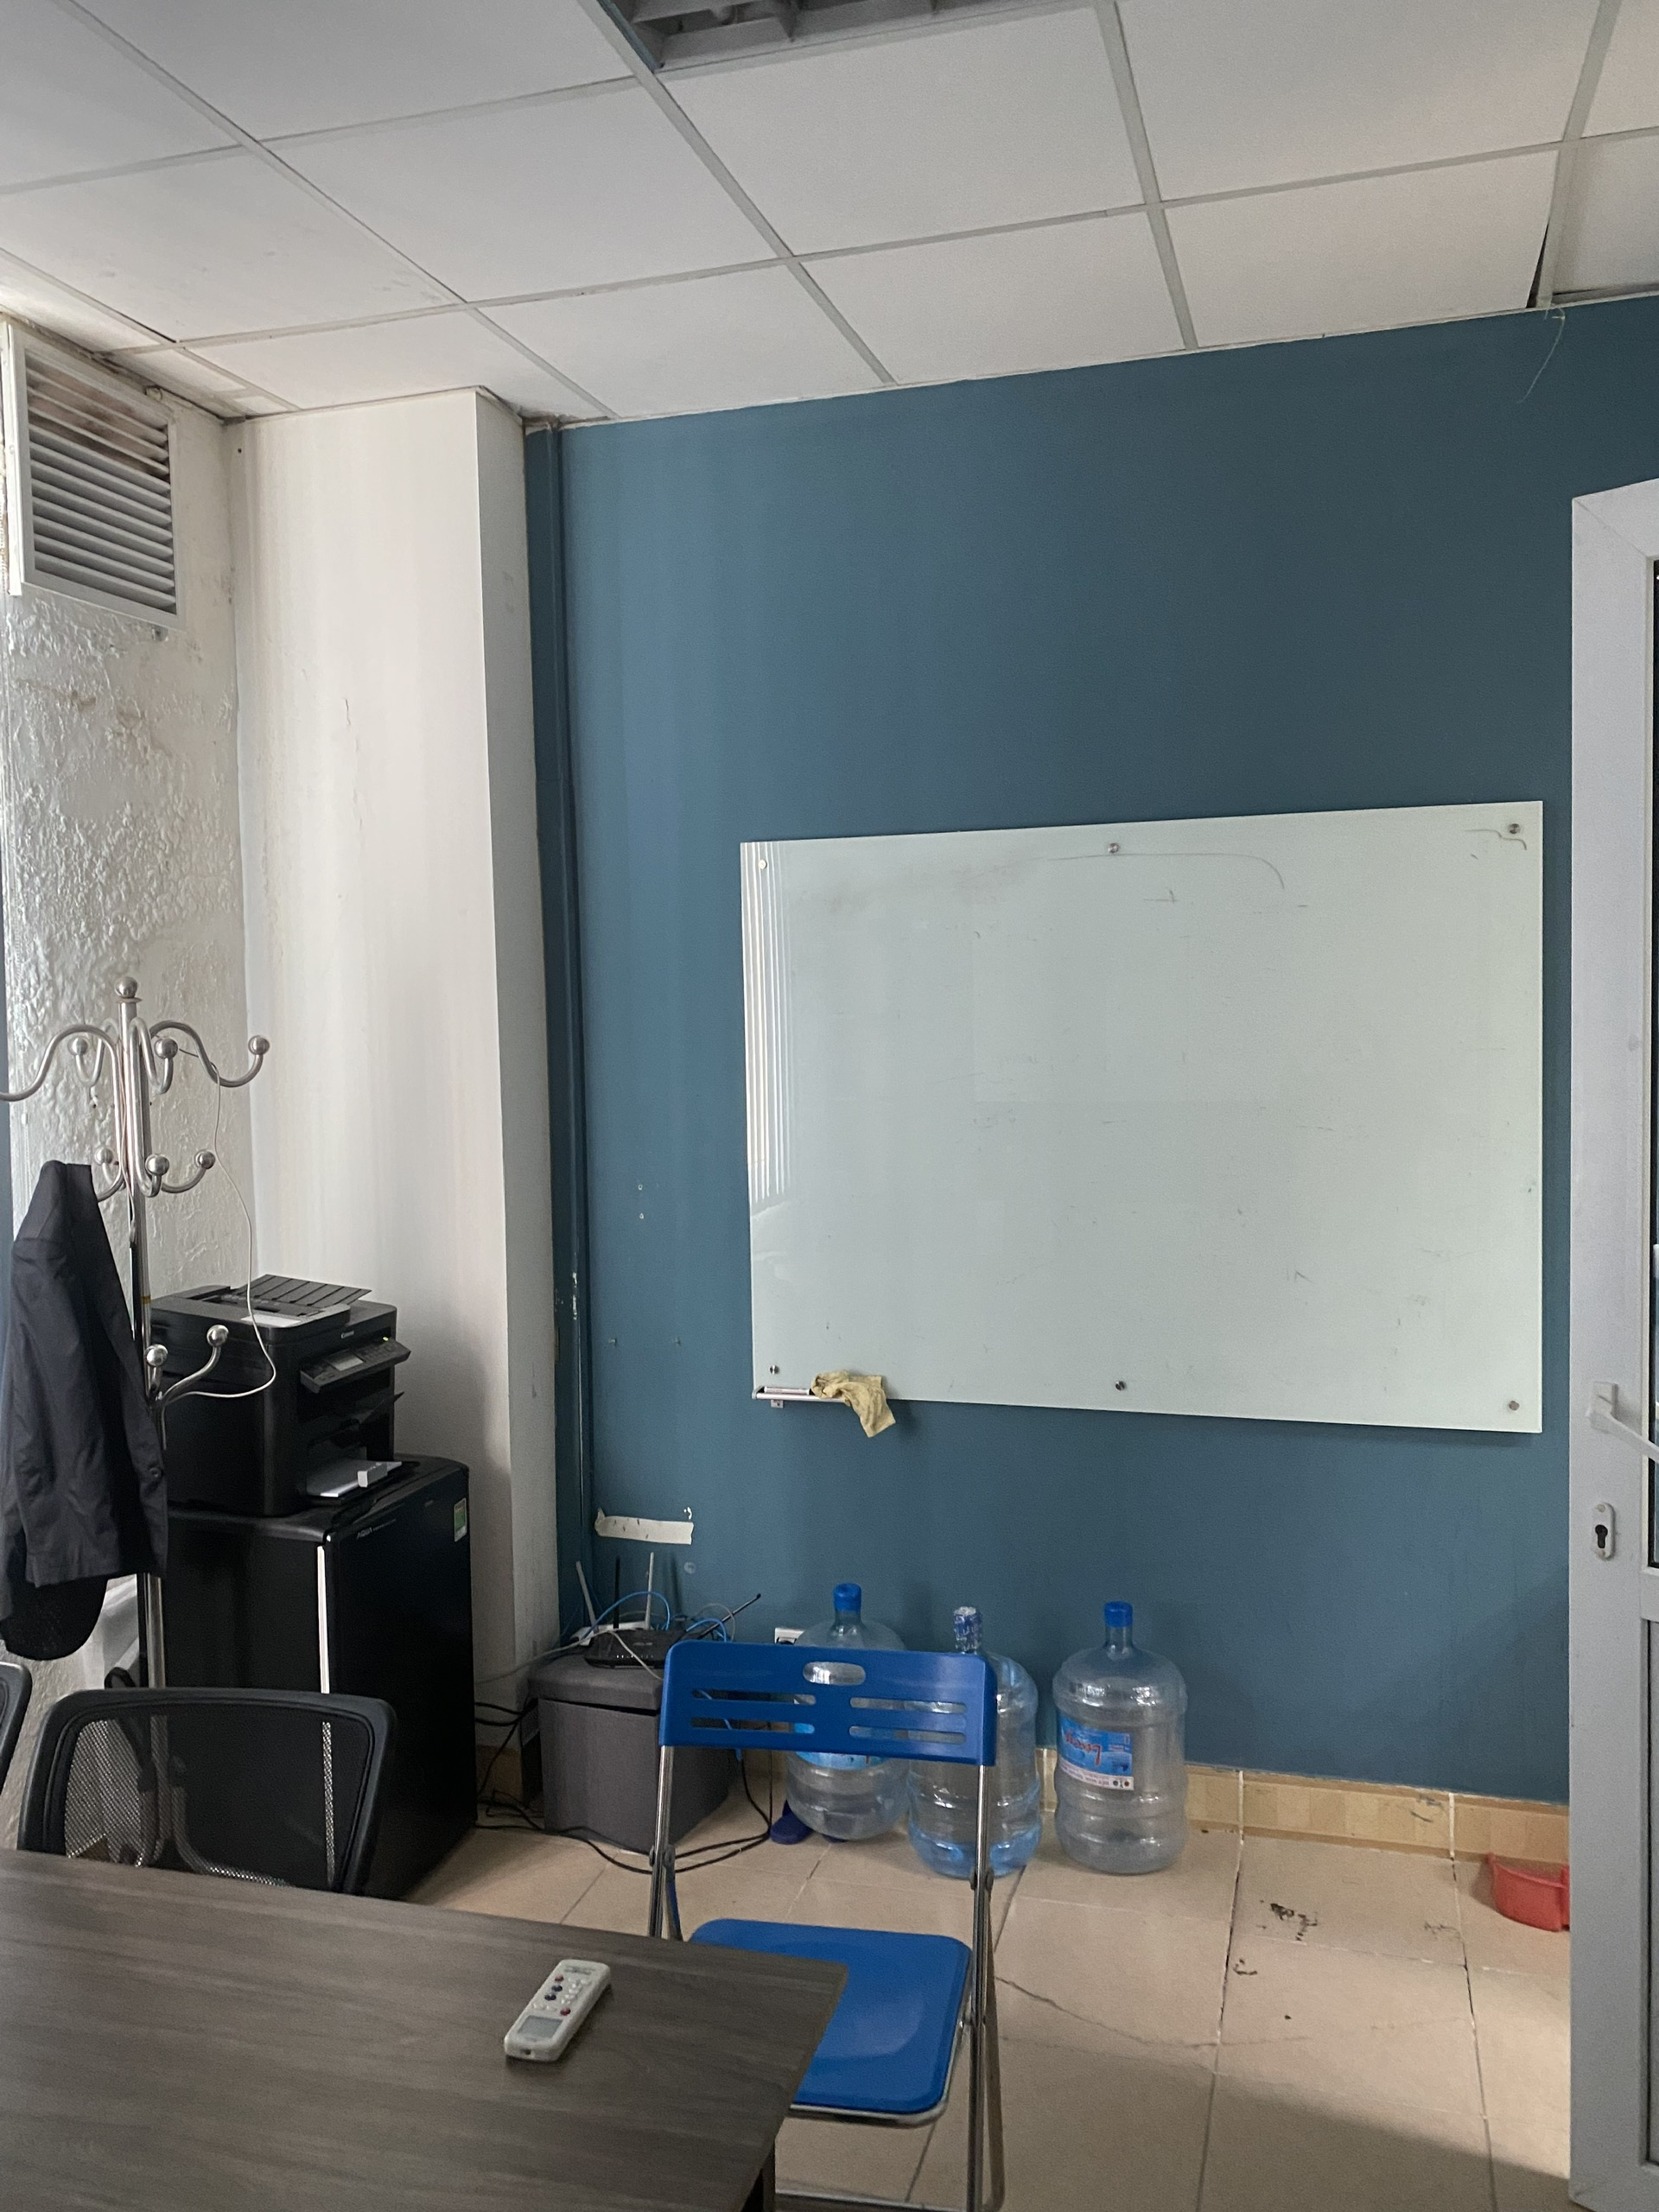
\includegraphics[width=0.6\linewidth]{Figure/small_room.jpg}
\caption{The small room.}
\label{fig:small_room}
\end{figure}

\begin{figure}[h!]
\centering
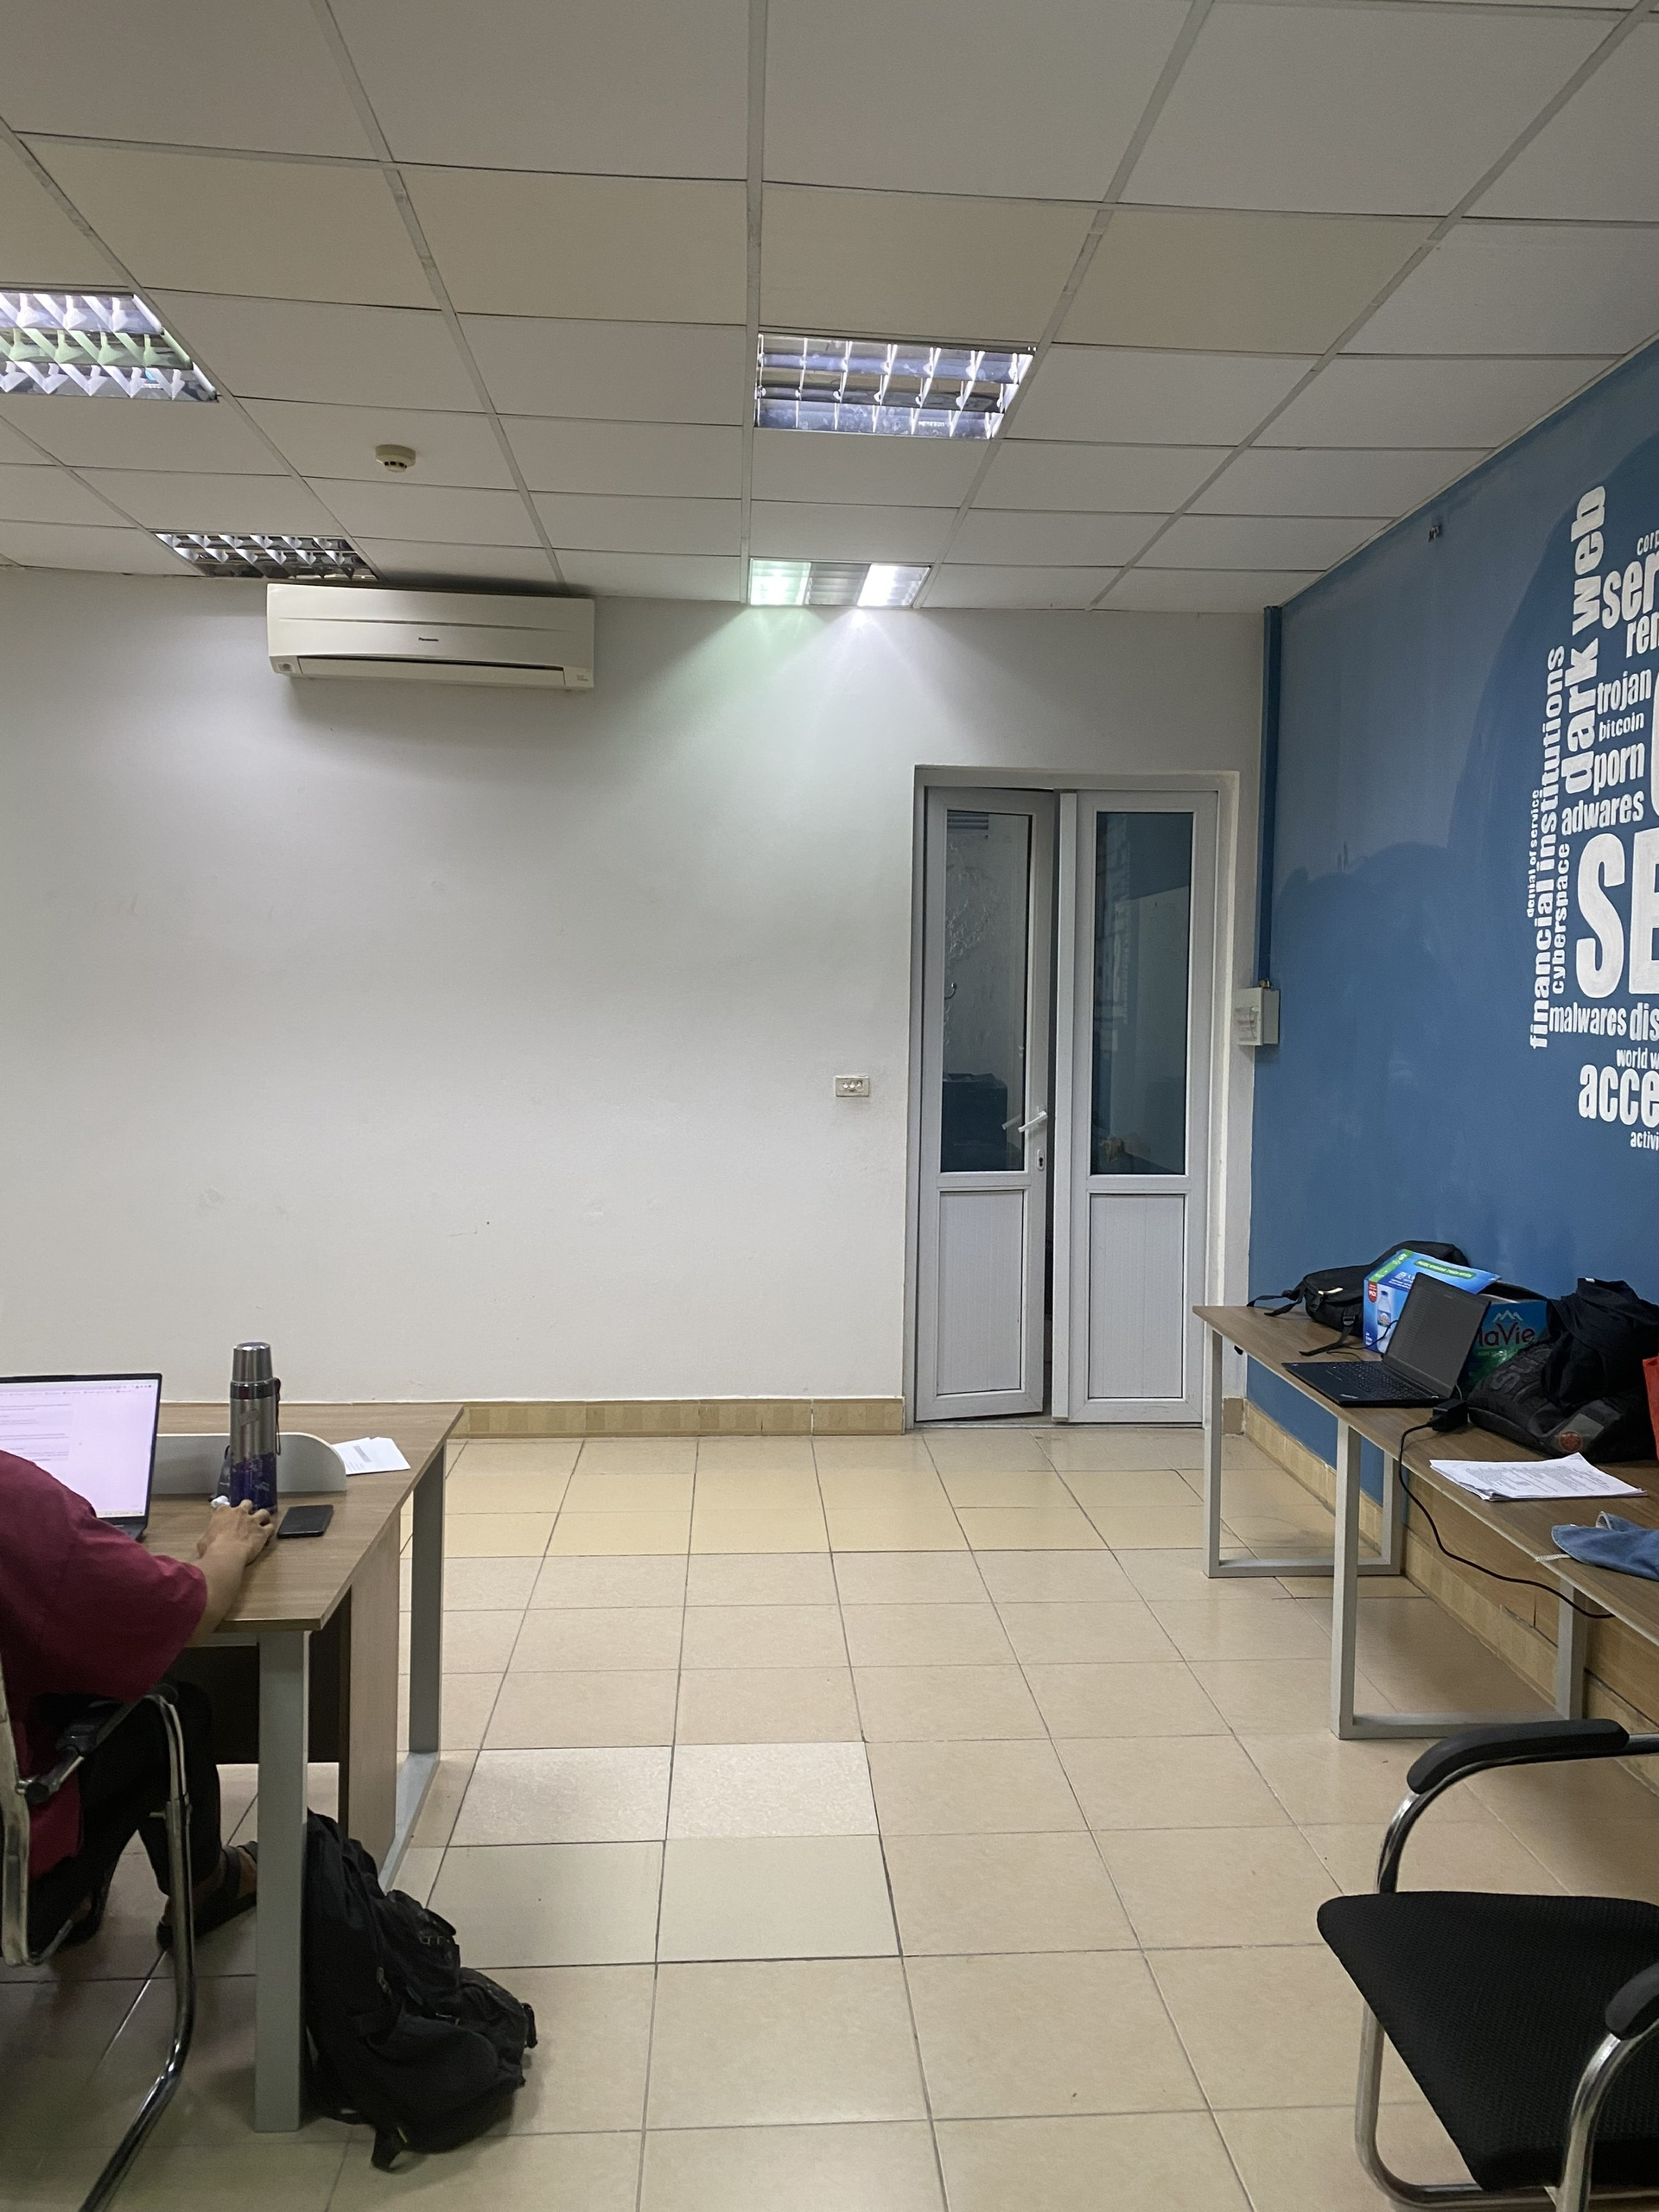
\includegraphics[width=0.6\linewidth]{Figure/large_room.jpg}
\caption{The large room.}
\label{fig:large_room}
\end{figure}

\begin{figure}[h!]
\centering
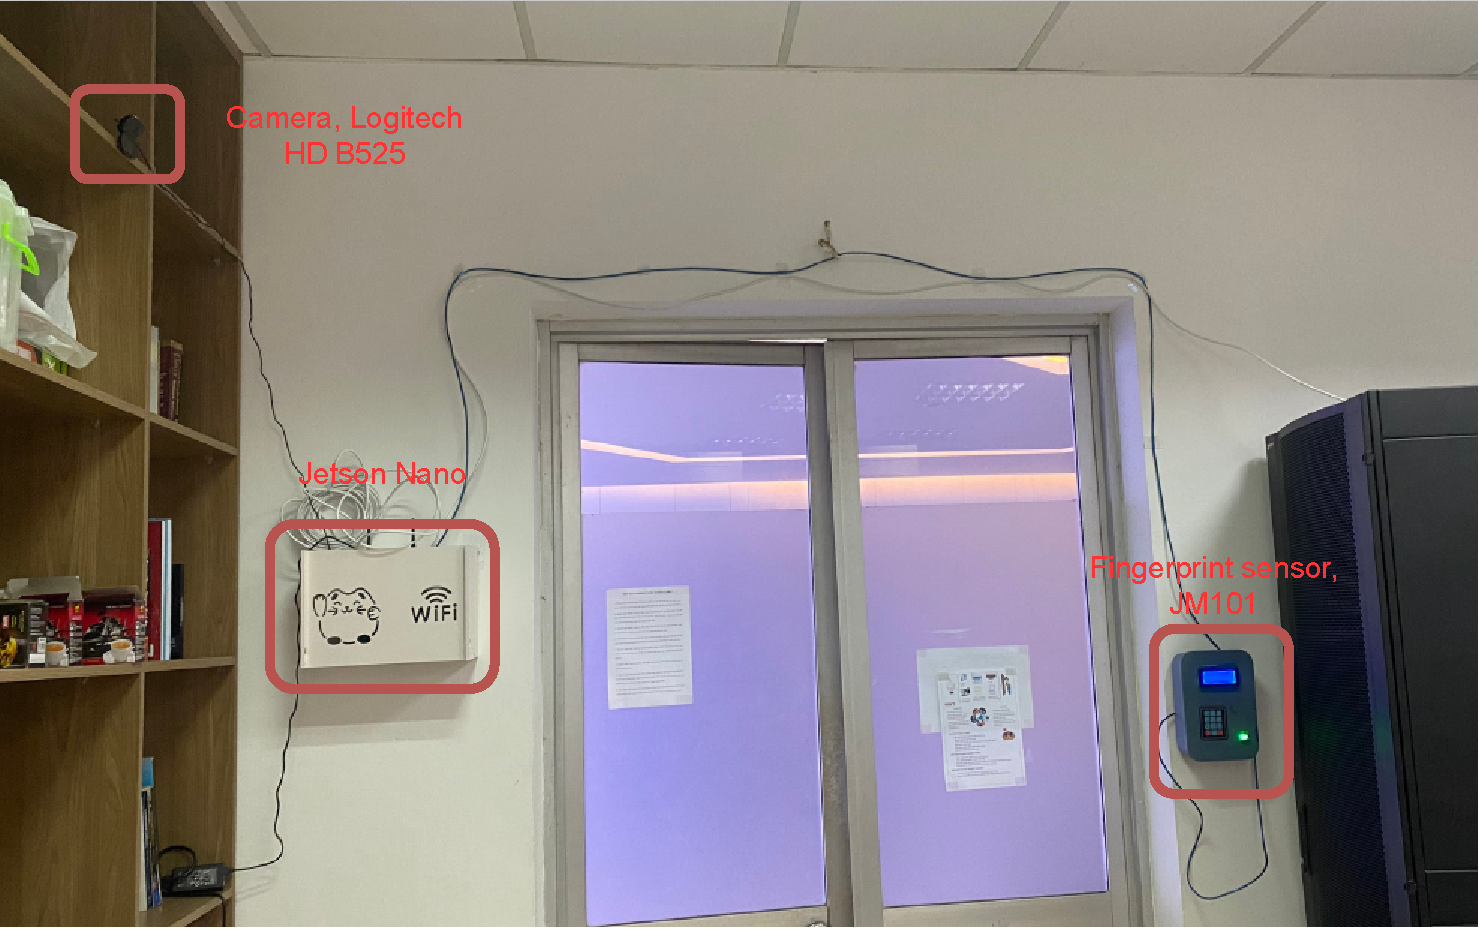
\includegraphics[width=\linewidth]{Figure/edge_door.pdf}
\caption{Deployment of entrance node.}
\label{fig:edge_door}
\end{figure}

\begin{figure}[h!]
\centering
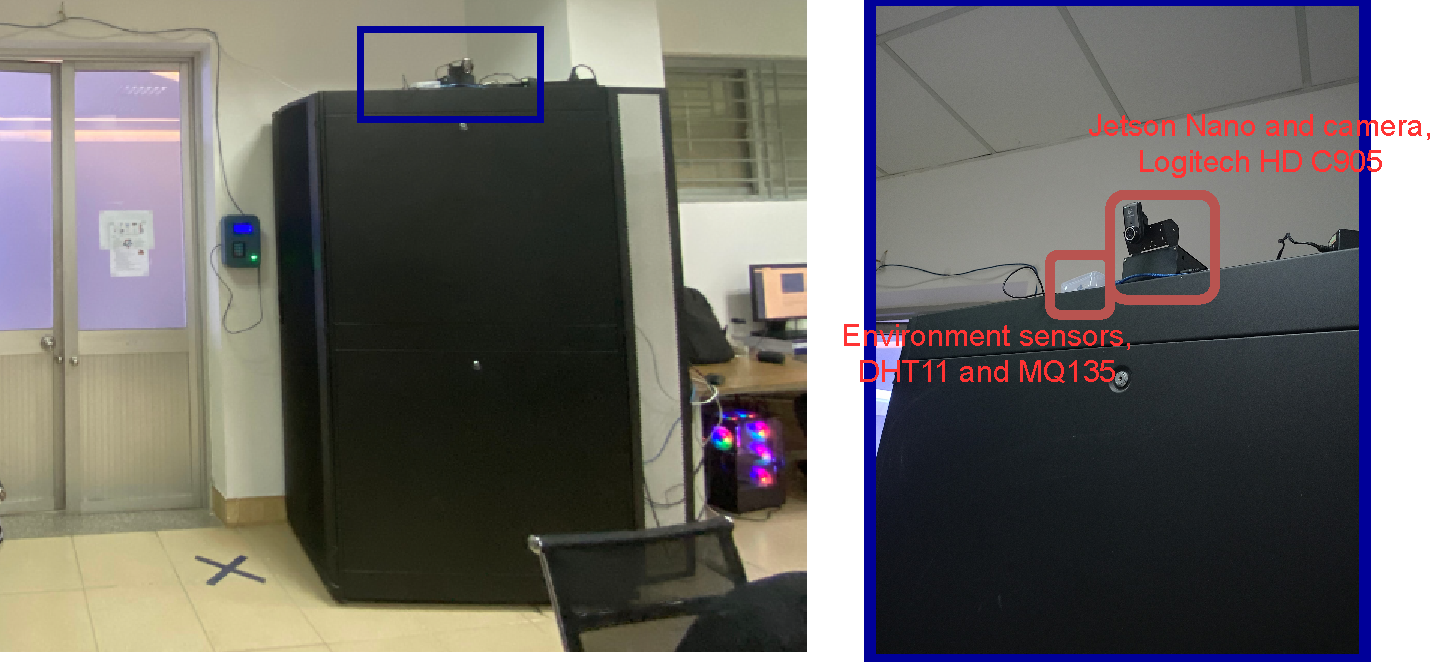
\includegraphics[width=\linewidth]{Figure/edge_largeroom.pdf}
\caption{Deployment of room node inside the large room.}
\label{fig:edge_largeroom}
\end{figure}

\begin{figure}[h!]
\centering
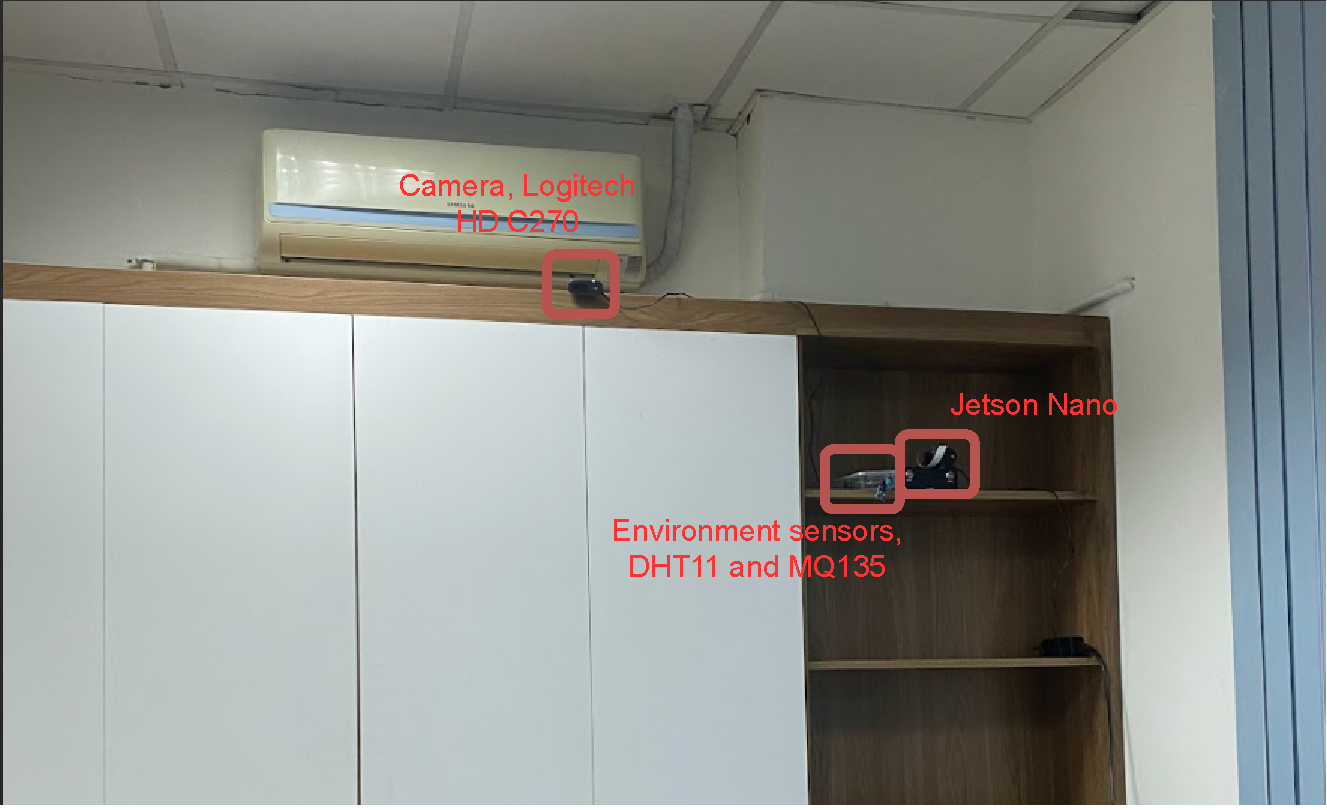
\includegraphics[width=\linewidth]{Figure/edge_smallroom.pdf}
\caption{Deployment of room node inside the small room.}
\label{fig:edge_smallroom}
\end{figure}

In each node inside the room, a USB camera and other peripheral devices will be connected to a Jetson Nano kit like in Figure~\ref{fig:device_combine}.

\begin{figure}[h!]
\centering
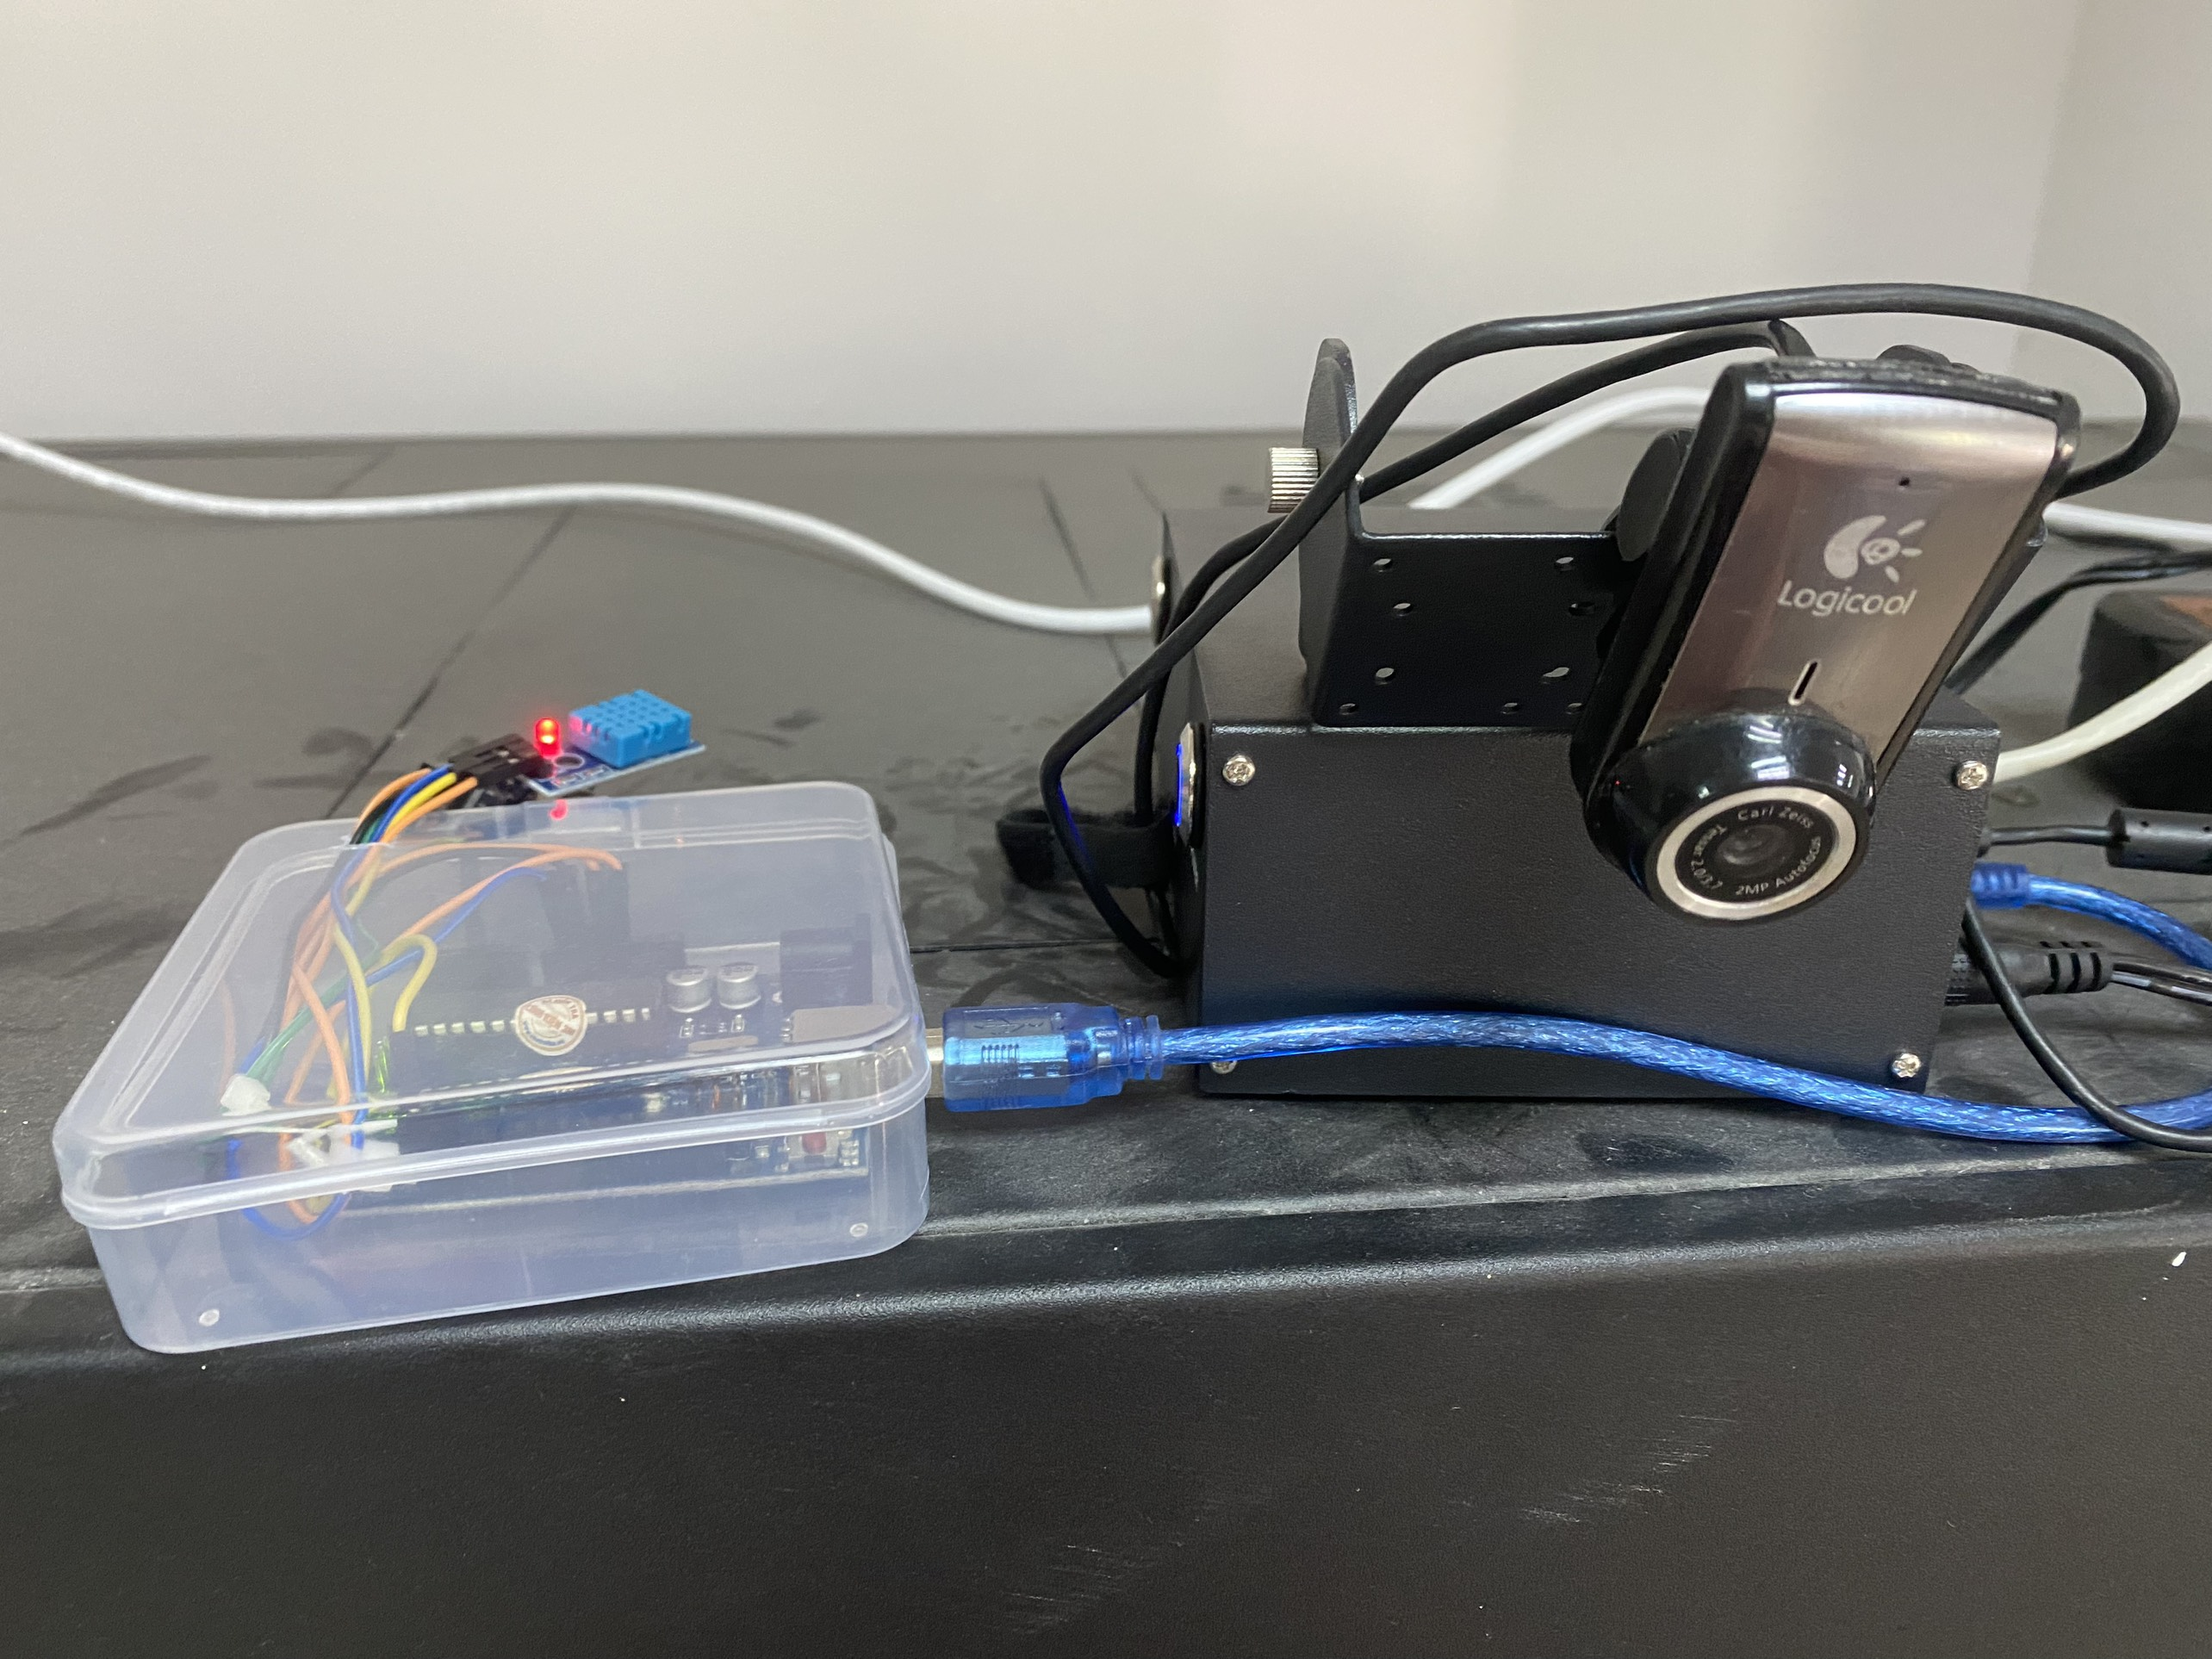
\includegraphics[width=0.8\linewidth]{Figure/devices_combine.jpg}
\caption{Jetson Nano with a camera and environment sensors.}
\label{fig:device_combine}
\end{figure}

\subsection{Operating speed experiments}
For further testing purposes, the speed test was conducted on Jetson Nano with the number of people inside the room increased. The overall testing frame rate of Jetson Nano is shown in Table~\ref{table:fps_test}. A single Jetson Nano conducted all the work including running two deep learning models and one tracking algorithm, receiving environment parameters from sensors and sending them with tracked human information each second, and sending raw input frames to the server every two seconds.

\begin{table}[h!]
\centering
\begin{tabular}{||c | c ||} 
\hline 
Number of people & FPS \\
\hline
0 & $34.4$ \\
1 & $25.1$ \\
2 & $20.9$ \\
3 & $17.1$ \\
4 & $15.1$ \\
5 & $13.0$ \\
6 & $11.2$ \\
7 & $9.6$ \\
\hline
\end{tabular}
\caption{FPS test results when increasing the number of people in a single camera frame.}
\label{table:fps_test}
\end{table}

When there were no more than two individuals present in the image, Jetson Nano was capable of achieving a frame rate greater than 20 FPS. However, as the number of individuals captured in the image increased, the frame rate also decreased. Specifically, starting from seven people, the FPS fell below 10. A significantly low frame rate can degrade the performance of the tracking algorithm~\cite{mabrouk2022assessment}. Therefore, for crowded scenarios, stronger hardware needs to be used or models and algorithms need to be further improved.

\subsection{Functionalities evaluation}
The functionalities of the AI module deployed on edge devices were evaluated through the output at the end application. The functionalities are shown by pictures of the user interface at the end application. Figure~\ref{fig:interface_overview} is a showcase of the interface of the application.

\begin{figure}[h!]
\centering
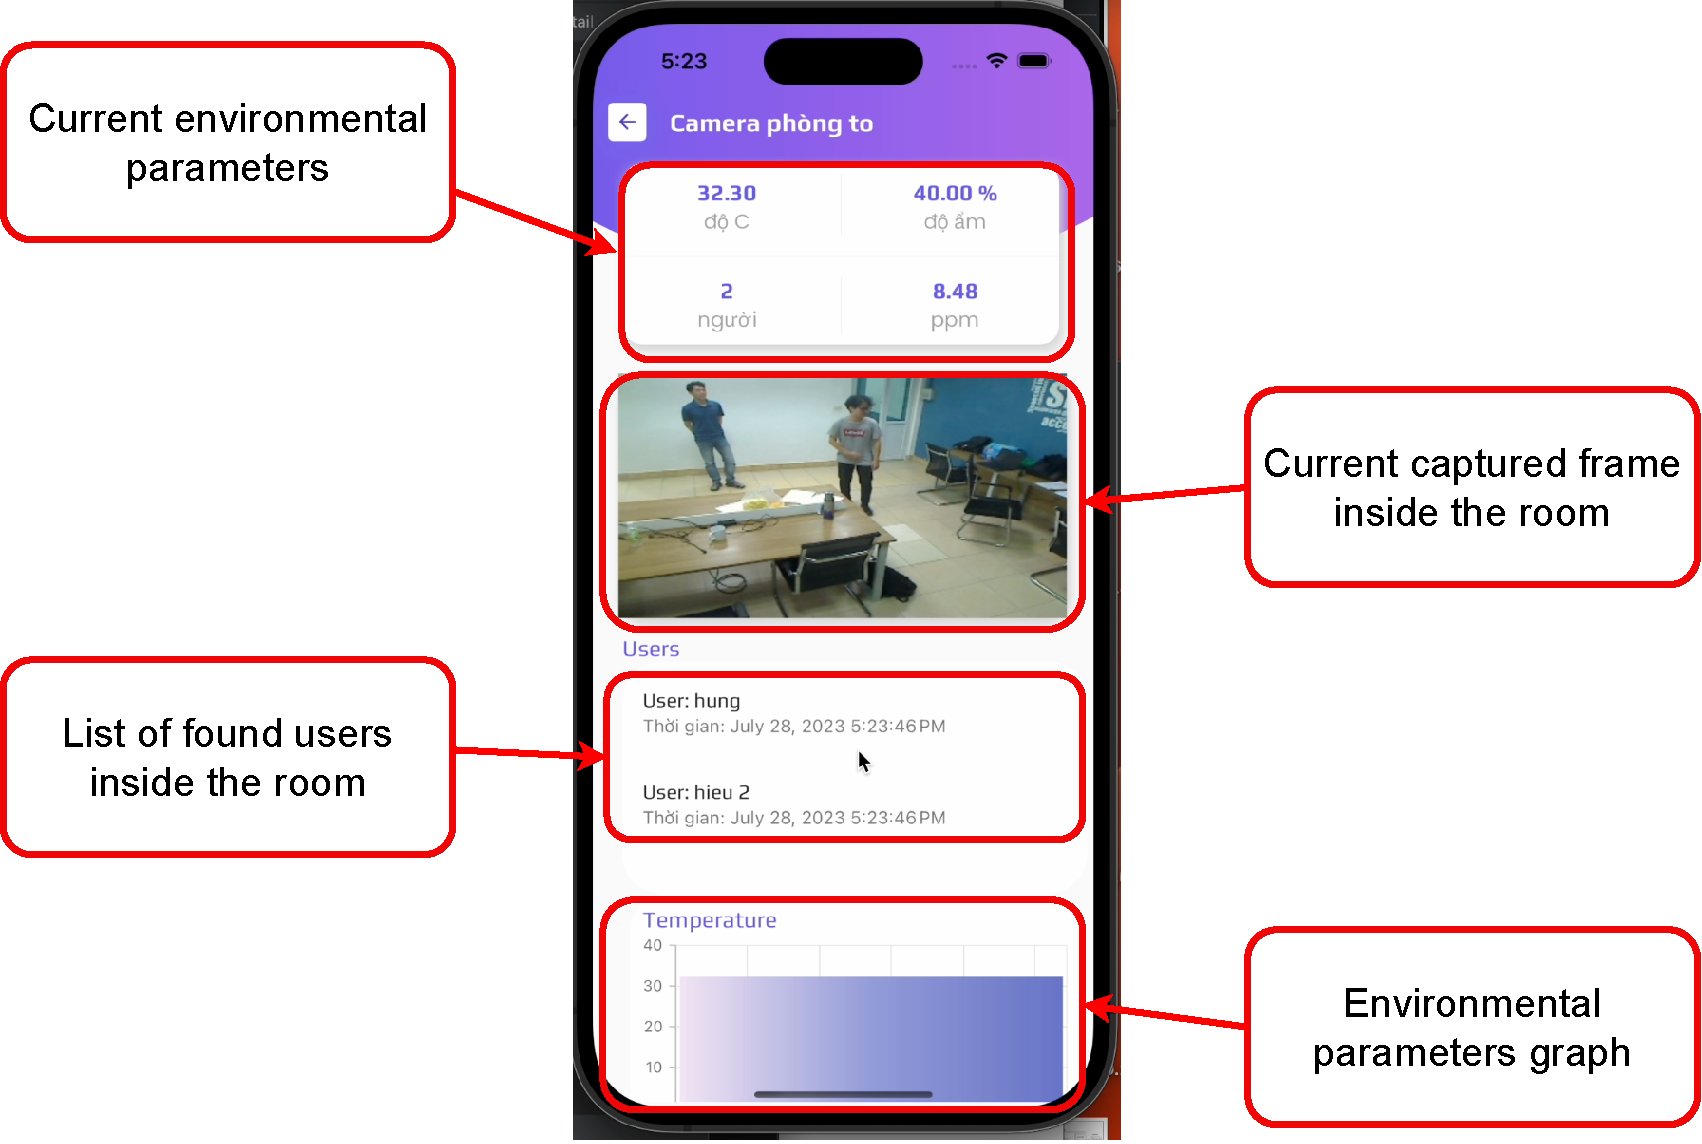
\includegraphics[width=\linewidth]{Figure/overview_interface.pdf}
\caption{The interface of the application.}
\label{fig:interface_overview}
\end{figure}

\subsubsection{Take attendance and identification when entering the room}
When a person checks attendance at the entrance by his or her fingerprint, the system will start to track that person inside the room. Figure~\ref{fig:func_enter} shows pictures of attendance checking and the result when a person enters the room. Jetson Nano can identify that person and send the information to the server.

\begin{figure}[h!]
\centering
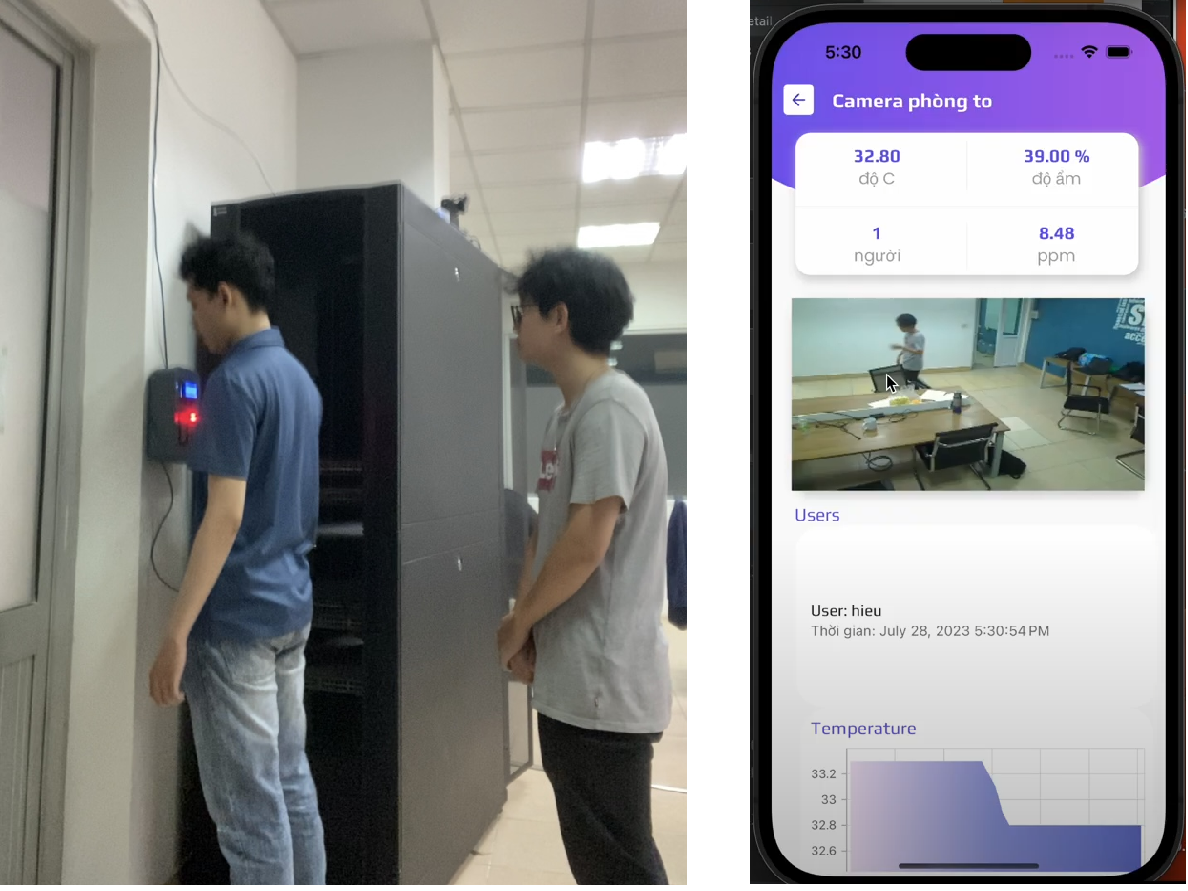
\includegraphics[width=\linewidth]{Figure/func_enter.pdf}
\caption{Attendance checking at entrance and interface of the application when there is a person entering the room.}
\label{fig:func_enter}
\end{figure}

\subsubsection{Re-ID when moving to another room}
The system re-identified people when they switched from the large room to the small room as shown in Figure~\ref{fig:func_switch}. All information including when a person entered the room, how they moved in the room, and which room they visited are all collected. This information was sent from multiple Jetson Nano and processed by the server.

\begin{figure}[h!]
\centering
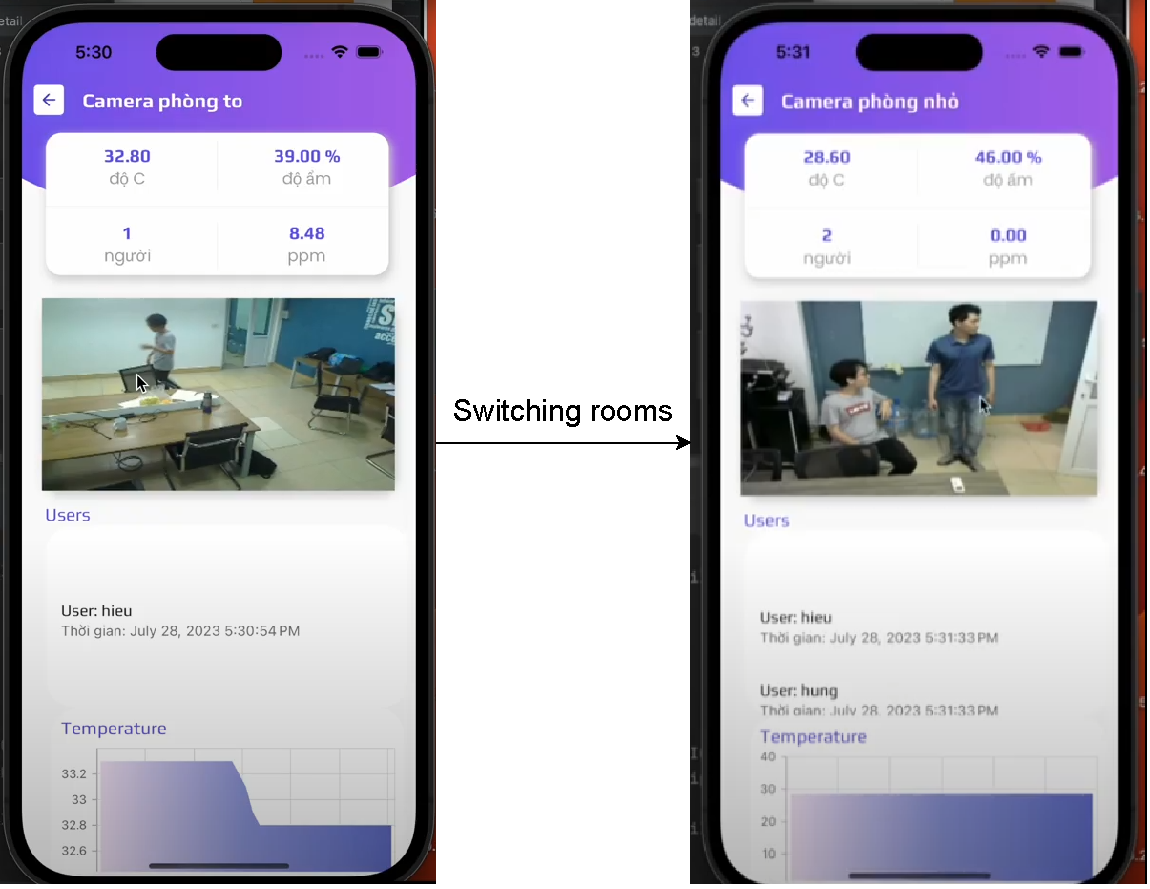
\includegraphics[width=\linewidth]{Figure/func_switch.pdf}
\caption{Results when switching rooms.}
\label{fig:func_switch}
\end{figure}

\subsubsection{Re-ID when disappearing from the frame for a period}
Sometimes, an object may obstruct a person from the camera's view. As an illustration in Figure~\ref{fig:func_disappear}, the person bent down to retrieve a pencil under a table and becomes obscured. When he reappeared after a short time, he was re-identified by the system. If a person disappears from all cameras for a long period of time, that person will be considered leaving the room.

\begin{figure}[h!]
\centering
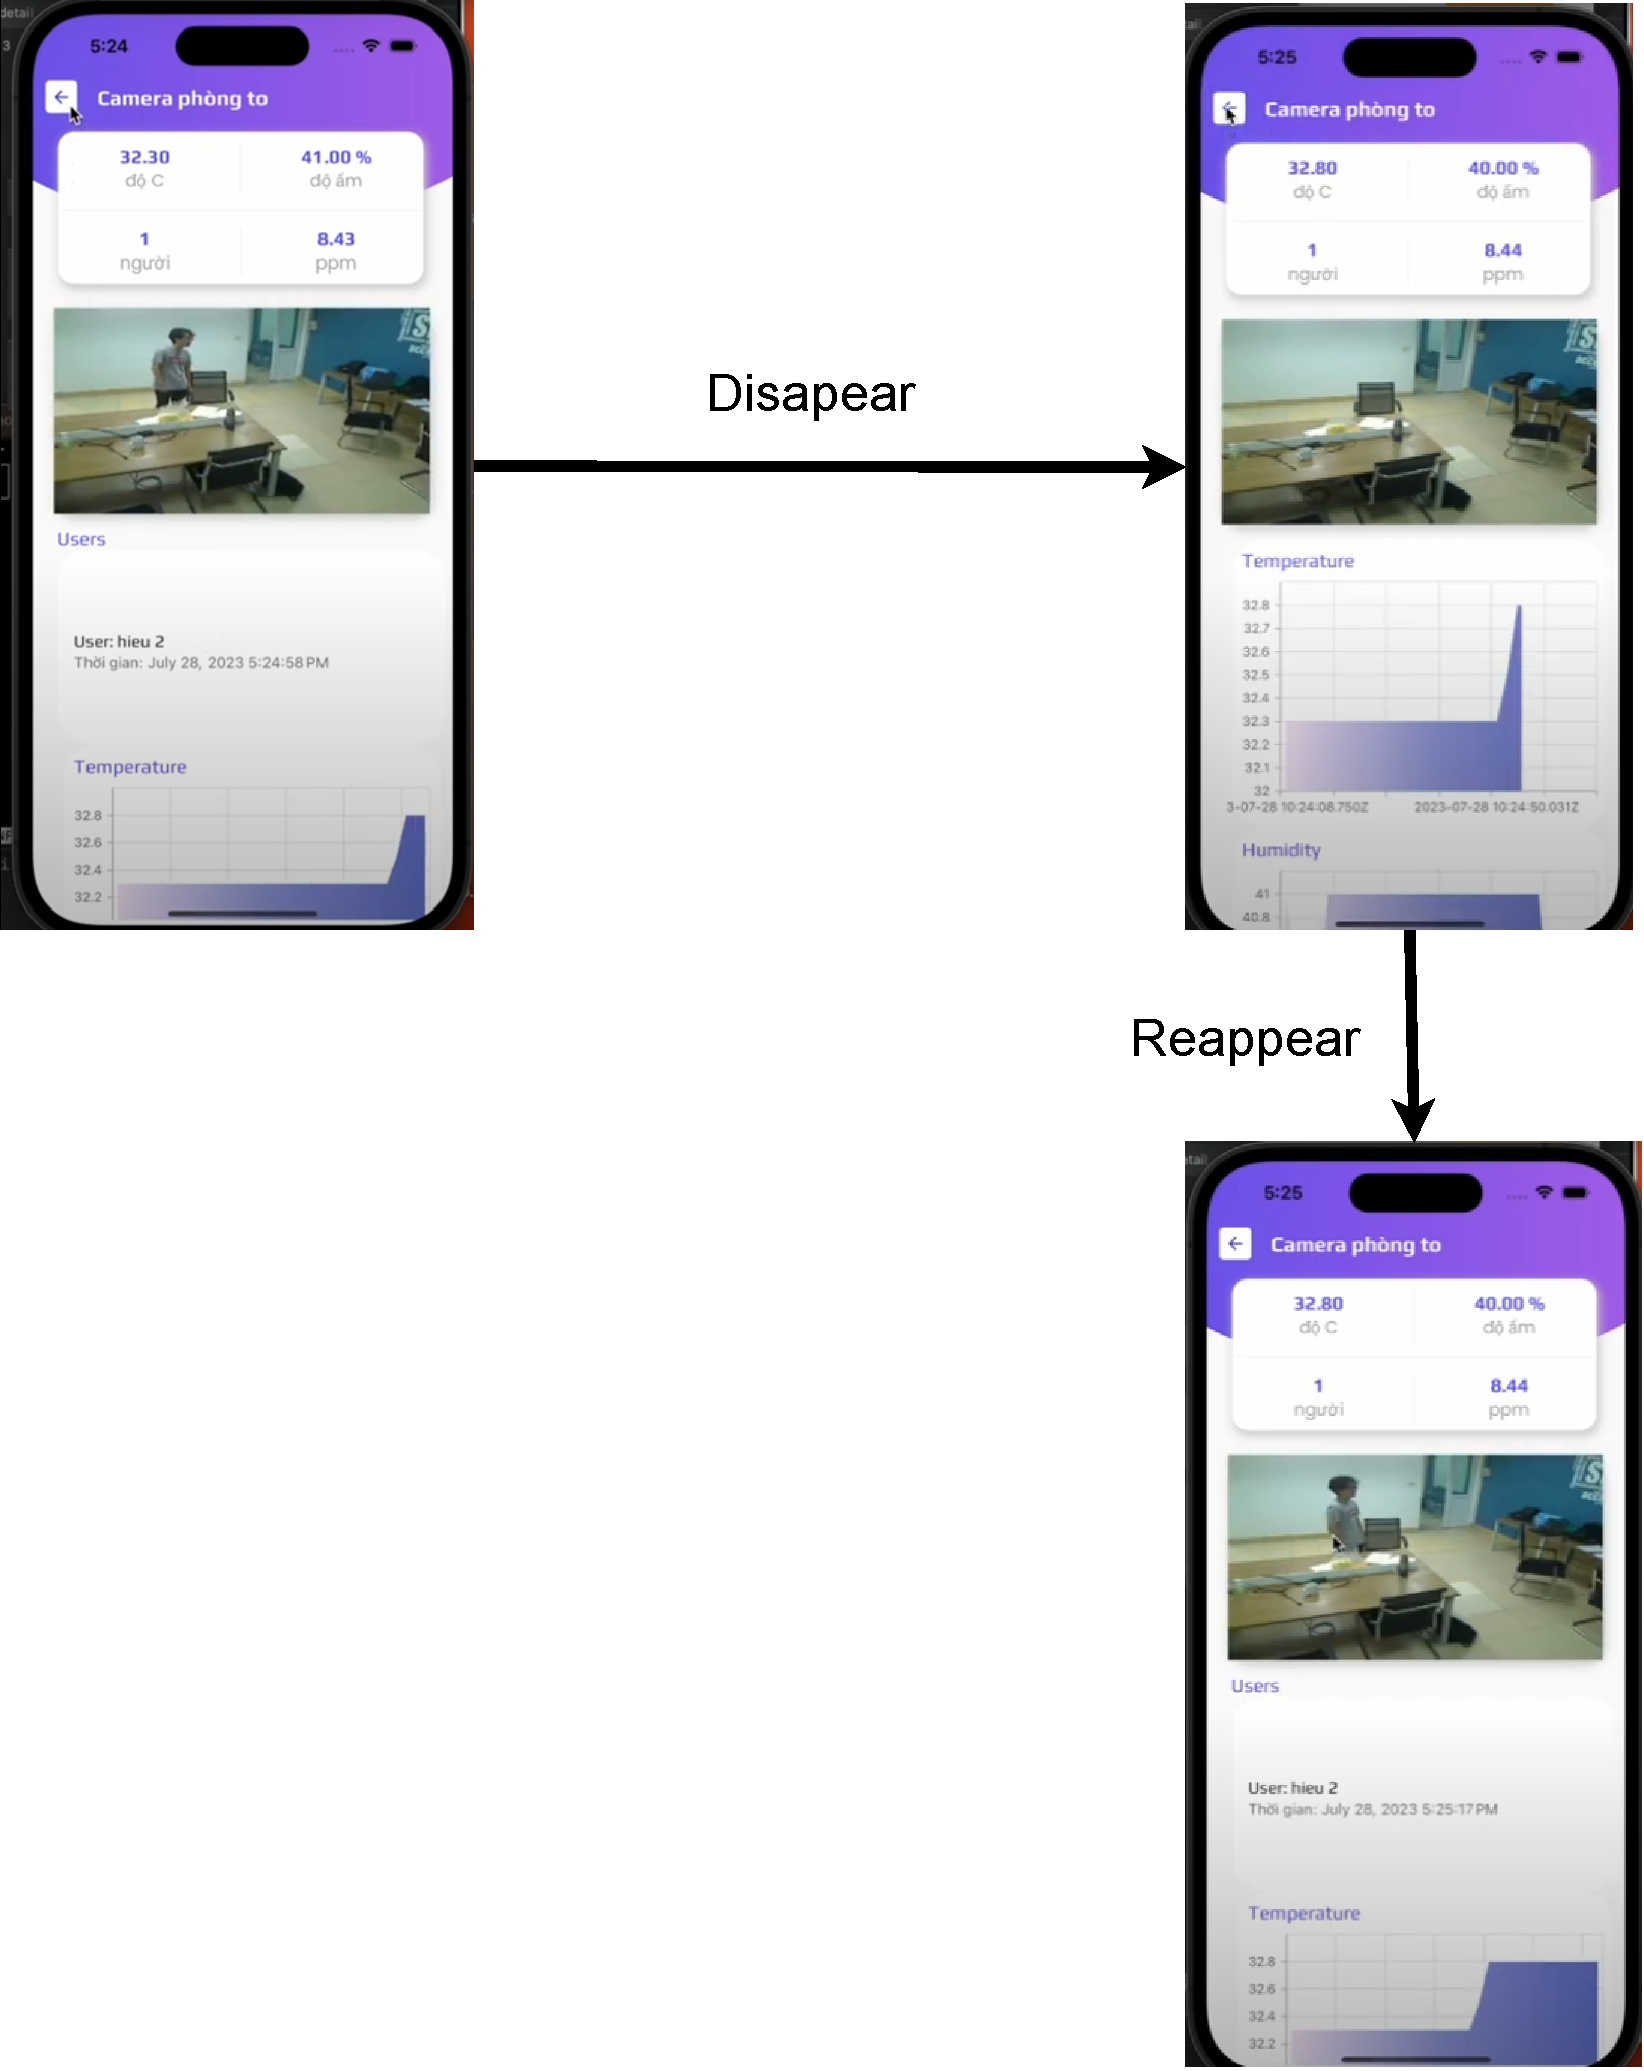
\includegraphics[width=\linewidth]{Figure/func_disappear.pdf}
\caption{Results when a person disappears from the frame from a period and reappears.}
\label{fig:func_disappear}
\end{figure}

\end{document}